% !TEX root = ./main.tex
%%%%%%%%%%%%%%%%%%%%%%%%%%%%%%%%%%%%%%%%%%%%%%%%%%%%%%%%%%%%%%%%%%%%%%%%%%%%%%%%%%%%%%%%%%
% Dans cette section, indiquez et décrivez tous les Invariants nécessaires.              %
%                                                                                        %
% Pour chaque SP nécessitant un Invariant (une sous-section/SP):                         %
% - Donnez l'Invariant Graphique                                                         %
% - Donnez l'Invariant Formel correspondant à l'Invariant Graphique                      %
% Pensez à utiliser les notations définies précédemment.                                 %
%%%%%%%%%%%%%%%%%%%%%%%%%%%%%%%%%%%%%%%%%%%%%%%%%%%%%%%%%%%%%%%%%%%%%%%%%%%%%%%%%%%%%%%%%%
\section{Invariants}\label{invariants}
%%%%%%%%%%%%%%%%%%%%

\subsection{Représentation de la Postcondition}
\\
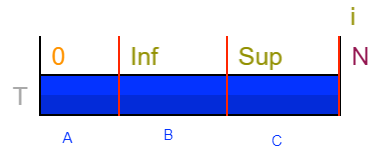
\includegraphics[width = 10cm]{invariant_EBZ952.png}
\newline
\noindent
\newline
Avec :\\\indent
A -> Déjà parcouru (sup \neq MAXPOS(T,0,inf) et \; inf \neq MINPOS(T,0,inf))\\\indent
B -> $$sum$ = SUM(T, Inf, Sup) , $inf$  = MINPOS(T,0,N)  et  $sup$  = MAXPOS(T,0,N)$\\\indent
C -> $Déjà parcouru (sup \neq MAXPOS(T,0,N) et \; inf \neq MINPOS(T,0,N)) $

\subsection{Représentation de l'invariant graphique}
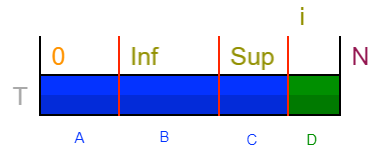
\includegraphics[width = 10 cm]{invariant.png}
\newline
\noindent

Avec :\\\indent
A ->  Déjà parcouru (sup \neq MAXPOS(T,0,inf) et \; inf \neq MINPOS(T,0,inf))\\\indent
B -> $$sum$ \; = SUM(T, Inf, Sup), inf = MINPOS(T, 0, i)  et sup = MAXPOS(T, 0, i)$\\\indent 
C -> $$new\_sum$ = NEWSUM(T,N,inf,sup)$ \\\indent 
D -> $Reste à parcourir$ 


\subsection{Invariant Formel}
\raggedright
T = T_0 \wedge  N =  N_0 \wedge 0 \leq inf \leq sup \leq N \wedge new\_sum = NEWSUM(T,N,min\_pos,max\_pos)  \wedge  $max\_pos$  = MAXPOS(T, 0, i) \wedge  $min\_pos$  = MINPOS(T, 0, i)
\wedge sum = SUM(T,N,min\_pos,max\_pos)
